\documentclass[a4paper,12pt,twoside]{memoir}

% Castellano
\usepackage[spanish,es-tabla]{babel}
\selectlanguage{spanish}
\usepackage[utf8]{inputenc}
\usepackage[T1]{fontenc}
\usepackage{lmodern} % Scalable font
\usepackage{microtype}
\usepackage{placeins}

\RequirePackage{booktabs}
\RequirePackage[table]{xcolor}
\RequirePackage{xtab}
\RequirePackage{multirow}

% Links
\PassOptionsToPackage{hyphens}{url}\usepackage[colorlinks]{hyperref}
\hypersetup{
	allcolors = {red}
}

% Ecuaciones
\usepackage{amsmath}

% Rutas de fichero / paquete
\newcommand{\ruta}[1]{{\sffamily #1}}

% Párrafos
\nonzeroparskip

% Huérfanas y viudas
\widowpenalty100000
\clubpenalty100000

% Imagenes
\usepackage{graphicx}
\newcommand{\imagen}[2]{
	\begin{figure}[!h]
		\centering
		\includegraphics[width=0.9\textwidth]{#1}
		\caption{#2}\label{fig:#1}
	\end{figure}
	\FloatBarrier
}

\newcommand{\imagenflotante}[2]{
	\begin{figure}%[!h]
		\centering
		\includegraphics[width=0.9\textwidth]{#1}
		\caption{#2}\label{fig:#1}
	\end{figure}
}



% El comando \figura nos permite insertar figuras comodamente, y utilizando
% siempre el mismo formato. Los parametros son:
% 1 -> Porcentaje del ancho de página que ocupará la figura (de 0 a 1)
% 2 --> Fichero de la imagen
% 3 --> Texto a pie de imagen
% 4 --> Etiqueta (label) para referencias
% 5 --> Opciones que queramos pasarle al \includegraphics
% 6 --> Opciones de posicionamiento a pasarle a \begin{figure}
\newcommand{\figuraConPosicion}[6]{%
  \setlength{\anchoFloat}{#1\textwidth}%
  \addtolength{\anchoFloat}{-4\fboxsep}%
  \setlength{\anchoFigura}{\anchoFloat}%
  \begin{figure}[#6]
    \begin{center}%
      \Ovalbox{%
        \begin{minipage}{\anchoFloat}%
          \begin{center}%
            \includegraphics[width=\anchoFigura,#5]{#2}%
            \caption{#3}%
            \label{#4}%
          \end{center}%
        \end{minipage}
      }%
    \end{center}%
  \end{figure}%
}

%
% Comando para incluir imágenes en formato apaisado (sin marco).
\newcommand{\figuraApaisadaSinMarco}[5]{%
  \begin{figure}%
    \begin{center}%
    \includegraphics[angle=90,height=#1\textheight,#5]{#2}%
    \caption{#3}%
    \label{#4}%
    \end{center}%
  \end{figure}%
}
% Para las tablas
\newcommand{\otoprule}{\midrule [\heavyrulewidth]}
%
% Nuevo comando para tablas pequeñas (menos de una página).
\newcommand{\tablaSmall}[5]{%
 \begin{table}
  \begin{center}
   \rowcolors {2}{gray!35}{}
   \begin{tabular}{#2}
    \toprule
    #4
    \otoprule
    #5
    \bottomrule
   \end{tabular}
   \caption{#1}
   \label{tabla:#3}
  \end{center}
 \end{table}
}

%
% Nuevo comando para tablas pequeñas (menos de una página).
\newcommand{\tablaSmallSinColores}[5]{%
 \begin{table}[H]
  \begin{center}
   \begin{tabular}{#2}
    \toprule
    #4
    \otoprule
    #5
    \bottomrule
   \end{tabular}
   \caption{#1}
   \label{tabla:#3}
  \end{center}
 \end{table}
}

\newcommand{\tablaApaisadaSmall}[5]{%
\begin{landscape}
  \begin{table}
   \begin{center}
    \rowcolors {2}{gray!35}{}
    \begin{tabular}{#2}
     \toprule
     #4
     \otoprule
     #5
     \bottomrule
    \end{tabular}
    \caption{#1}
    \label{tabla:#3}
   \end{center}
  \end{table}
\end{landscape}
}

%
% Nuevo comando para tablas grandes con cabecera y filas alternas coloreadas en gris.
\newcommand{\tabla}[6]{%
  \begin{center}
    \tablefirsthead{
      \toprule
      #5
      \otoprule
    }
    \tablehead{
      \multicolumn{#3}{l}{\small\sl continúa desde la página anterior}\\
      \toprule
      #5
      \otoprule
    }
    \tabletail{
      \hline
      \multicolumn{#3}{r}{\small\sl continúa en la página siguiente}\\
    }
    \tablelasttail{
      \hline
    }
    \bottomcaption{#1}
    \rowcolors {2}{gray!35}{}
    \begin{xtabular}{#2}
      #6
      \bottomrule
    \end{xtabular}
    \label{tabla:#4}
  \end{center}
}

%
% Nuevo comando para tablas grandes con cabecera.
\newcommand{\tablaSinColores}[6]{%
  \begin{center}
    \tablefirsthead{
      \toprule
      #5
      \otoprule
    }
    \tablehead{
      \multicolumn{#3}{l}{\small\sl continúa desde la página anterior}\\
      \toprule
      #5
      \otoprule
    }
    \tabletail{
      \hline
      \multicolumn{#3}{r}{\small\sl continúa en la página siguiente}\\
    }
    \tablelasttail{
      \hline
    }
    \bottomcaption{#1}
    \begin{xtabular}{#2}
      #6
      \bottomrule
    \end{xtabular}
    \label{tabla:#4}
  \end{center}
}

%
% Nuevo comando para tablas grandes sin cabecera.
\newcommand{\tablaSinCabecera}[5]{%
  \begin{center}
    \tablefirsthead{
      \toprule
    }
    \tablehead{
      \multicolumn{#3}{l}{\small\sl continúa desde la página anterior}\\
      \hline
    }
    \tabletail{
      \hline
      \multicolumn{#3}{r}{\small\sl continúa en la página siguiente}\\
    }
    \tablelasttail{
      \hline
    }
    \bottomcaption{#1}
  \begin{xtabular}{#2}
    #5
   \bottomrule
  \end{xtabular}
  \label{tabla:#4}
  \end{center}
}



\definecolor{cgoLight}{HTML}{EEEEEE}
\definecolor{cgoExtralight}{HTML}{FFFFFF}

%
% Nuevo comando para tablas grandes sin cabecera.
\newcommand{\tablaSinCabeceraConBandas}[5]{%
  \begin{center}
    \tablefirsthead{
      \toprule
    }
    \tablehead{
      \multicolumn{#3}{l}{\small\sl continúa desde la página anterior}\\
      \hline
    }
    \tabletail{
      \hline
      \multicolumn{#3}{r}{\small\sl continúa en la página siguiente}\\
    }
    \tablelasttail{
      \hline
    }
    \bottomcaption{#1}
    \rowcolors[]{1}{cgoExtralight}{cgoLight}

  \begin{xtabular}{#2}
    #5
   \bottomrule
  \end{xtabular}
  \label{tabla:#4}
  \end{center}
}



\graphicspath{ {./img/} }

% Capítulos
\chapterstyle{bianchi}
\newcommand{\capitulo}[2]{
	\setcounter{chapter}{#1}
	\setcounter{section}{0}
	\setcounter{figure}{0}
	\setcounter{table}{0}
	\chapter*{#2}
	\addcontentsline{toc}{chapter}{#2}
	\markboth{#2}{#2}
}

% Apéndices
\renewcommand{\appendixname}{Apéndice}
\renewcommand*\cftappendixname{\appendixname}

\newcommand{\apendice}[1]{
	%\renewcommand{\thechapter}{A}
	\chapter{#1}
}

\renewcommand*\cftappendixname{\appendixname\ }

% Formato de portada
\makeatletter
\usepackage{xcolor}
\newcommand{\tutor}[1]{\def\@tutor{#1}}
\newcommand{\course}[1]{\def\@course{#1}}
\definecolor{cpardoBox}{HTML}{E6E6FF}
\def\maketitle{
  \null
  \thispagestyle{empty}
  % Cabecera ----------------
\noindent
\includegraphics[width=\textwidth]{cabecera}\vspace{1cm}%
  \vfill
  % Título proyecto y escudo informática ----------------
  \colorbox{cpardoBox}{%
    \begin{minipage}{.8\textwidth}
      \vspace{.5cm}\Large
      \begin{center}
      \textbf{TFG del Grado en Ingeniería Informática}\vspace{.6cm}\\
      \textbf{\LARGE\@title{}}
      \end{center}
      \vspace{.2cm}
    \end{minipage}

  }%
  \hfill\begin{minipage}{.20\textwidth}
    
\includegraphics[width=\textwidth]{escudoInfor}
  \end{minipage}
  \vfill
  % Datos de alumno, curso y tutores ------------------
  \begin{center}%
  {%
    \noindent\LARGE
    Presentado por \@author{}\\ 
    en Universidad de Burgos --- \@date{}\\
    Tutores: \@tutor{}\\
  }%
  \end{center}%
  \null
  \cleardoublepage
  }
\makeatother

\newcommand{\nombre}{Alberto Porres Fernández} %%% cambio de comando

% Datos de portada
\title{Plataforma de Corrección Automática de Ejercicios en Python}
\author{\nombre}
\tutor{Bruno Baruque Zanón\\ y Roberto Carlos Casado Vara}
\date{7 de julio de 2022}

\begin{document}

\maketitle


\newpage\null\thispagestyle{empty}\newpage


%%%%%%%%%%%%%%%%%%%%%%%%%%%%%%%%%%%%%%%%%%%%%%%%%%%%%%%%%%%%%%%%%%%%%%%%%%%%%%%%%%%%%%%%
\thispagestyle{empty}


\noindent
\includegraphics[width=\textwidth]{cabecera}\vspace{1cm}

\noindent D. Bruno Baruque Zanón, profesor del Departamento de Ingeniería Informática, Área de Ciencia de la Computación e Inteligencia Artificial, y D. Roberto Carlos Casado Vara, profesor del departamento de Matemáticas y Computación, Área de Matemática Aplicada.

\noindent Exponen:

\noindent Que el alumno D. \nombre, con DNI 71708167D, ha realizado el Trabajo final de Grado en Ingeniería Informática titulado Plataforma de Corrección Automática de Ejercicios en Python. 

\noindent Y que dicho trabajo ha sido realizado por el alumno bajo la dirección del que suscribe, en virtud de lo cual se autoriza su presentación y defensa.

\begin{center} %\large
En Burgos, {\large 7 de julio de 2022}
\end{center}

\vfill\vfill\vfill

% Author and supervisor
\begin{minipage}{0.45\textwidth}
\begin{flushleft} %\large
Vº. Bº. del Tutor:\\[2cm]
D. Bruno Baruque Zanón
\end{flushleft}
\end{minipage}
\hfill
\begin{minipage}{0.45\textwidth}
\begin{flushleft} %\large
Vº. Bº. del co-tutor:\\[2cm]
D. Roberto Carlos Casado Vara
\end{flushleft}
\end{minipage}
\hfill

\vfill

% para casos con solo un tutor comentar lo anterior
% y descomentar lo siguiente
%Vº. Bº. del Tutor:\\[2cm]
%D. nombre tutor


\newpage\null\thispagestyle{empty}\newpage




\frontmatter

% Abstract en castellano
\renewcommand*\abstractname{Resumen}
\begin{abstract}
En la formación de alumnos sobre programación se necesita lograr que estos desarrollen pensamiento algorítmico desde un principio. En ese marco, los cursos online de iniciación a la programación encuentran un importante espacio de formación en la actualidad pues en los últimos tiempos se ha popularizado el aprendizaje en línea y el autoaprendizaje.

En este proyecto se ha realizado el desarrollo de una plataforma orientada a la enseñanza online que permita presentar a los alumnos contenidos teóricos y, principalmente, ejercicios prácticos. La mayor ventaja de la plataforma es la corrección automática de las soluciones a los ejercicios programadas por los alumnos, de forma transparente al profesor.

\end{abstract}

\renewcommand*\abstractname{Descriptores}
\begin{abstract}
Enseñanza-aprendizaje, autograding (evaluación automática), programación para principiantes.
\end{abstract}

\clearpage

% Abstract en inglés
\renewcommand*\abstractname{Abstract}
\begin{abstract}
When training students in programming, it is necessary to ensure that they develop algorithmic thinking from the very beginning. In this context, online courses for programming initiation find an important training space nowadays, since online learning and self-learning have become more popular in recent times.

In this project, the development of a platform oriented to online teaching has been carried out, which allows presenting theoretical contents and, mainly, practical exercises to the students. The main advantage of the platform is the automatic correction of the solutions to the exercises programmed by the students, in a transparent way to the teacher.
\end{abstract}

\renewcommand*\abstractname{Keywords}
\begin{abstract}
Teaching-learning, autograding (automatic grading), programming for beginners.
\end{abstract}

\clearpage

% Indices
\tableofcontents

\clearpage

\listoffigures

\clearpage

\listoftables
\clearpage

\mainmatter
\capitulo{1}{Introducción}

Una de las caraterísticas del hombre es su capacidad para el desempeño de tareas complejas. Para llegar a desarrollarlas los individuos tienen que pasar en la mayoría de las ocasiones por un proceso de formación y adiestramiento, pues la simple observación, la intuición, la imitación, etc, por sí solas no suelen lograr que se alcance objetivo o nivel pretendido de conocimientos, habilidades y desempeño. Por esta razón, en todas las sociedades humanas evolucionadas la formación se contempla como uno de sus cimientos más importantes.

Los elementos básicos que componen el proceso de formación-aprendizaje son bien conocidos: el alumno, el profesor, el método de enseñanza y la evaluación. Existen además otros factores como los soportes y sistemas que constituyen el entorno de proceso: el lugar, la forma de trasmistir presencial, a distancia, telemática, en directo, en diferido, con apoyos gráficos, textuales, experimentales, etc.
Este proyecto se ha enfocado en la evaluación de la enseñanza de la programación informática para alumnos principiantes. La corrección de ejercicios de programación puede suponer un trabajo lento y tedioso, que resta tiempo al profesor en su tarea de enseñanza y que puede demorar que el alumno conozca cuál es el resultado de los ejercicios realizados. En definitiva, es un sistema costoso.

Con un diseño adecuado de ejercicios y pruebas sobre los mismos se puede conseguir implementar una corrección automatizada (y rápida) de las respuestas de los alumnos. Éstos además, usando las pruebas proporcionadas por el profesor, pueden ir modificando sus respuestas antes de realizar la entrega final de sus ejercicios. Todo ello redunda en beneficios en el proceso de enseñanaza-aprendizaje: el alumno puede ir comprobando si ha diseñado o no un código que da el resultado esperado, el profesor tiene más tiempo para dedicar a la enseñanza y, se reduce el coste de evaluación.

El presente proyecto desarrolla una plataforma online que se enmarca en el anterior contexto. Permite al profesor poner a disposición de los estudiantes tanto los contenidos de los temas a tratar como tareas que los estudiantes han de resolver relacionadas con tales contenidos. Estos, cuando completan los ejercicios de programación propuestos, los entregan a través de la plataforma y obtienen automáticamente los resultados a la evaluación de sus respuestas.

\begin{figure}[h]
    \centering
    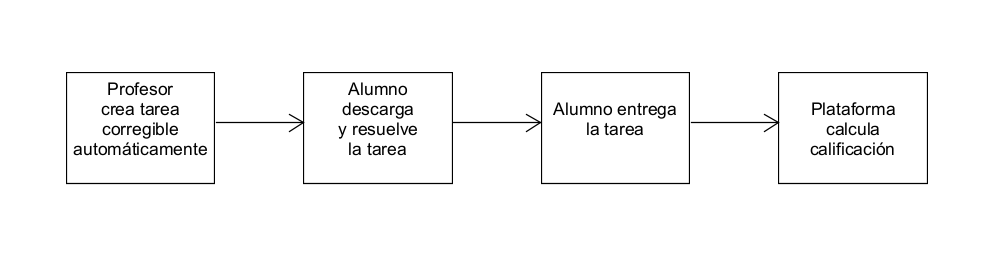
\includegraphics[width=\textwidth]{img/imgs-memoria/FuncionamientoBase.PNG}
    \caption{Funcionamiento Base}
\end{figure}
\capitulo{2}{Objetivos del proyecto}

En este apartado se van a detallar los objetivos que se han perseguido durante la realización de este proyecto, dividiéndose estos en objetivos generales, objetivos técnicos y objetivos personales.

\section{Objetivos generales}

\begin{itemize}
  \item Explorar diversas herramientas orientadas a la corrección automática
  de ejercicios en Python.
  \item Seleccionar una herramienta de corrección automática de ejercicios en Python.
  \item Desarrollar una plataforma web orientada a la enseñanza la cual permita corregir de forma automática ejercicios en Python a través de la herramienta seleccionada.
  \item Diseñar un sencillo curso introductorio a Python con sus respectivas tareas autocorregibles y alojarlo en la plataforma.
\end{itemize}


\section{Objetivos técnicos}
\begin{itemize}
  \item Crear una plataforma online para la comodidad de acceso a los usuarios de esta mediante Python y Flask.
  \item Corregir de forma automática ejercicios en Python dentro de la plataforma contenidos en Notebooks de Jupyter.
  \item Permitir la creación de tareas desde la propia web mediante la ejecución de Jupyter Notebook de forma remota.
  \item Alojar el código de la plataforma dentro de un contenedor Docker para posibilitar su posterior despliegue.
  \item Adaptar la herramienta de autocorrección seleccionada (Nbgrader) para el uso específico dado en la plataforma.
   
\end{itemize}

\section{Objetivos personales}

\begin{itemize}
  \item Ofrecer una base introductoria al aprendizaje del lenguaje de programación Python.
  \item Descubrir y manejar herramientas para el desarrollo de ejercicios autocorregibles en ambientes de programación.
  \item Descubrir y manejar herramientas para la creación de entornos web.
  \item Llevar a la práctica diversos conceptos teóricos estudiados como la metodología Agile, el control de versiones durante el desarrollo de un proyecto y el trabajo en equipo.
  \item Aplicar una metodología Agile al desarrollo del proyecto.
  \item Utilizar Git como sistema de control de versiones durante el desarrollo del proyecto.
 
\end{itemize}
\capitulo{3}{Conceptos teóricos}

En este apartada van a ser expuestos los conceptos teóricos pertenecientes a este proyecto y su desarrollo:

\section{Proceso de enseñanza - aprendizaje}
En la formación de individuos se suele hablar como un todo del proceso de enseñanza-aprendizaje\cite{EnsenanzaAprendizaje}. ¿En qué consiste este proceso? Empezaremos por definir los elementos que lo componen.

\subsection{Proceso de enseñanza}
Esta parte del proceso corresponde a las tareas de trasmisión de contenidos y conocimientos desarrolladas por el docente, para el que representa una de sus actividades más importante.

El profesor tiene en cuenta los contenidos de la materia que imparte y las estrategias didácticas para enseñar al alumno lo que ha de aprender, así como asistirle y encauzar su labor de aprendizaje. El docente modula lo que el alumno debe ir aprendiendo y cómo hacerlo, y acompaña el aprendizaje del estudiante. 


\subsection{Proceso de aprendizaje}
De acuerdo con la teoría de Piaget (1969)\cite{Piaget}\cite{Libro:Piaget}, el pensamiento es la base en la que se asienta el aprendizaje, es la manera de manifestarse la inteligencia. La inteligencia desarrolla una estructura y un funcionamiento. El propio funcionamiento modifica la estructura de la inteligencia y existe un interacción entre el individuo y el medio.

En cuanto al proceso de aprendizaje, las ideas principales de esta teoría son:

\begin{itemize}
\item El estudiante es quien lleva a cabo el aprendizaje. El profesor es un orientador o facilitador.
\item Para el aprendizaje de cualquier materia se requiere una continuidad o secuencia lógica y psicológica.
\item Han de respeterse las diferencias individuales entre los diferentes estudiantes.
\end{itemize}

Por parte del docente la enseñanza debe ser vista como el proceso de una relación personal con el estudiante en su viaje por el aprendizaje.

Es necesario comprender que el aprendizaje es personal, centrado en objetivos y, además, que precisa de constante retroalimentación. El aprendizaje debe basarse en una satisfactoria interacción entre los dos elementos principales que participan en el proceso: docente y estudiante.

Tanto el aprendizaje como la enseñanza son procesos que se presentan continuamente en la vida de todo ser humano, y no es posible hablar de ellos separadamente, pues forman una unidad conjunta.

El proceso de enseñanza-aprendizaje está compuesto por cuatro elementos: el profesor, el estudiante, la materia o contenido y los métodos didácticos. Cada uno de estos elementos influye en mayor o menor medida, dependiendo del modo en que se relacionan en un contexto determinado.

Al analizar cada uno de estos cuatro elementos, se identifican variables que influyen en el proceso enseñanza-aprendizaje:

\begin{itemize}
\item Docente: actitud, capacidad, relación con el estudiante, conocimientos de la materia, conocimientos/destrezas técnico-didácticos,  compromiso con el proceso…
\item Estudiante:  interés-motivación, capacidad, velocidad de aprendizaje, conocimientos previos, posición socioeconómica, dedicación…  
\item Materias/contendidos: complejidad, significado, importancia, relevancia práctica, interés general, proyección, …
\item Métodos didácticos: modo de presentación, técnicas-recursos-apoyos utilizados por el docente, dinámicas, actividades, sistemas de evaluación, realimentación de información sobre la evalución… 
\end{itemize}

\section{Evaluación}
El proceso de enseñanza-aprendizaje implica una variedad diferente de elementos, entre los cuales en este trabajo fin de grado nos centramos en la evaluación y la retroalimentación de información.

El tiempo de los profesores se tiene que distribuir entre varias tareas diferentes, entre las que destaca la enseñanza de conocimientos, la cual es imprescindible para dirigir a los alumnos al objetivo deseado. Cuanto mayor calidad tenga y mayor tiempo se dedique a esta actividad mejores resultados se podrán obtener en el proceso de enseñanza-aprendizaje. No obstante, los profesores pueden llegar a dedicar grandes cantidades de tiempo en actividades de corrección.

Durante las clases el profesor tiene multitud de formas de apoyar el aprendizaje de los alumnos. Una de las fundamentales es la resolución de dudas planteadas durante sus clases, lo que puede tener mucha importancia en cuestiones de difícil comprensión. 

Pero no siempre estas dudas son de igual interés para todos los alumnos y se plantea que hay alumnos o grupos que precisan un apoyo más personalizado, dedicando el profesor tiempo a tutorías y asistencia fuera del tiempo de clase. El estado actual de la tecnología ha incidido en la atención individual mediante la posibilidad de comentarios a través del uso de plataformas web y preguntas por correo electrónico. El profesorado puede dar así respuestas muy precisas y personalizadas de forma rápida.

Los profesores dedican algo de tiempo a resolver las preguntas individuales de los estudiantes y, a pesar de que esto no es muy popular, constituye una excelente manera de superar cursos difíciles. Con el advenimiento de la tecnología, la evaluación individual ha crecido significativamente. Los profesores ahorran tiempo en la recuperación de comentarios mediante el uso de plataformas web y los estudiantes se benefician enormemente de esto, ya que reciben respuestas rápidas y precisas. 

Cuando se trata de realizar la evaluación a  textos complejos de los alumnos, o temas en cuya respuesta importa el desarrollo o la interpretación como la historia o la literatura es difícil recurrir a la tecnología. Sin embargo, en no pocos casos y sobre todo en áreas técnicas, se ha conseguido una mejoría en los métodos de evaluación, reduciendo la cantidad de tiempo invertida corrigiendo. Aparte de los típicos test de evaluación a través de plataformas informáticas, destacan también los sistemas de evaluación automatizada o autograding para corrección en plataformas de enseñanza de programación.


\section{Evaluación de código informático}
En la generación de código informático para cualquier ejercicio que se plantee se suele encontrar que existe gran libertad y posibilidades de llegar al mismo resultado con diferente código. A la hora de corregir, el profesor se encuentra con dos tipos de evaluación de dicho código:

\begin{itemize}
\item En primer lugar la evaluación o corrección funcional: comprueba que el código hace realmente el trabajo solicitado, con independencia de la calidad de ese código. Es decir, si el código es eficaz para lograr el resultado.
\item En segundo lugar, existe un valoración no funcional. Aquí entran el estilo de programación, la claridad y legibilidad del código, el uso eficiente de recursos como la memoria, el tiempo de ejecución, redundancia de código, etc.
\end{itemize}

El evaluador normalmente tiene que dar un peso a cada una de estas formas de evaluación del código. No obstante, cuando se trata de programación para principiantes, las cuestiones de estilo y eficacia no suelen considerarse importantes. Es decir, corresponde aplicar sobre todo la evaluación funcional pues lo que se requiere es que el alumno llegue a conocer y manejar los elementos de lenguaje, sintaxis, estructura, funciones básicas, etc.

Para alumnos principiantes se diseñan ejercicios que requieren programas muy simples para enseñarles los conceptos básicos de la programación. Se trata de ejercicios relativamente sencillos cuya corrección es también bastante rápida. Sin embargo, el volumen de los ejercicios puede ser significativo. Si sumamos a esto que en los estadios iniciales de programación el número de alumnos inscritos suele ser elevado, el volumen de ejercicios a corregir puede llegar a ser muy alto además de tedioso. Esto ha llevado a que aparezcan enfoques nuevos para tratar de ayudar en el proceso.

\section{Autograding}
Los autograders (también denominados autoevaluadores o evaluadores automáticos) son herramientas que permiten a los profesores la evaluación automatizada de código. Su uso es bastante amplio en cursos de informática e ingeniería. También puede encontrarse en otras ramas afines como ciencia de datos y estadística e, incluso, se llega a utilizar en áreas no relacionadas con la informática.

Su uso ahorra tiempo en la calificación, en especial cuando se trata de cursos con gran número de alumnos inscritos. Ofrecen a los alumnos la evaluación de los ejercicios en tiempo real e idealmente pueden proporcionarles retroalmentación de sus resultados y/o comentarios para que puedan servirles en las siguientes etapas de su proceso de aprendizaje.

Su forma de uso común es medir la calidad del código generado por el alumno como respuesta a ejercicios propuestos mediante la comparación de los resultados de la ejecución de dicho código con el resultado esperado o la respuesta que proporciona el código de referencia que el profesor establezca como solución. Se obtendrá una calificación basada en el resultado de tal comparación.

El profesor prueba de este modo la habilidad del estudiante en los casos de programación planteados. Se puede implementar de modo que sea el estudiante el que en línea aplique el autograding y compruebe si su código es o no correcto. Asimismo otra implementación común es que el alumno envíe sus respuestas al profesor, que será quien aplique el programa de evaluación automática para obtener las calificaciones de cada alumno de grupo en los distintas tareas de ejercicios encomendadas al alumnado.


























\capitulo{4}{Técnicas y herramientas}

Esta parte de la memoria tiene como objetivo presentar las técnicas metodológicas y las herramientas de desarrollo que se han utilizado para llevar a cabo el proyecto.

\section{Metodología de desarrollo: Agile}

El desarrollo de este proyecto se ha llevado a cabo siguiendo la Métodología Agile\cite{MetodologiaAgile} derivada del manifiesto Agile\cite{ManifiestoAgile}. Esta metodología de diseño software busca un desarrollo de proyectos que precisan rapidez y flexibilidad, proponiendo una filosofía de trabajo y organización diferente a los métodos tradicionales en la que el proyecto es dividido en pequeñas tareas que han de ser completadas en marcas de tiempo predefinidas. Estos periodos de tiempo son denominados Sprints y, en el caso de este proyecto, cada sprint ha tenido una duración de 14 días.

\section{Control de versiones: GitHub}

Se denomina control de versiones a la técnica de gestión de los cambios que un producto o proyecto sufre a lo largo de todo su desarrollo. En el caso de este proyecto se ha utilizado la herramienta GitHub \cite{tool:GitHub}, la cual es una plataforma de desarrollo colaborativo para alojar proyectos mediante el sofwate de control de versiones Git.

Puede consultarse el repositorio correspondiente a este proyecto en la URL \url{https://github.com/AlbertoPorres/autograder-python}.

\section{Gestión y seguimiento de tareas: ZenHub}

ZenHub\cite{tool:ZenHub} es una extensión de la herramienta de control de versiones GitHub que ofrece un manejo agile de los proyectos, con el fin de ayudar a los equipos de desarrollo con la organización de tareas y flujo de trabajo.


\section{Servidor / Back-End}

\subsection{Python}
Python\cite{tool:Python} es un lenguaje de programación de alto nivel, interpretado, flexible, orientado a objetos y caracterizado por su fácil comprensión y aprendizaje. Python es un lenguaje de uso general por lo que ofrece una gran cantidad de usos como la creación de aplicaciones web, scripts, automatización de procesos y la creación de módulos de aprendizaje automático.

\subsection{Nbgrader}
Nbgrader\cite{tool:Nbgrader} es una librería de Python que facilita la creación y calificación de tareas en notebooks de Jupyter. Permite a los instructores crear fácilmente tareas basadas en el notebook que incluyen tanto ejercicios de codificación como respuestas libres escritas. Nbgrader también proporciona una interfaz optimizada para calificar rápidamente las tareas completadas.

En este proyecto y, una vez consideradas diversas herramientas de autocorrección de ejercicios, se tomó la decisión de utilizar Nbgrader como autograder dentro del proyecto. Esto es debido a la sencilla e intuitiva usabilidad que ofrece y a la ausencia de problemas en los procesos de instalación y ejecución que otras herramientas consideradas inicialmente sí presentaban.

Su implementación en el Back-End ha consistido en el uso de su API para las labores de calificación automática y generación de tareas corregibles automáticamente.

\subsection{Flask}
Flask\cite{tool:Flask} es un microframework de desarrollo de aplicaciones web escrito en Python y basado en el patrón arquitectural Modelo - Vista - Controlador. Este está diseñado con el objetivo de hacer del desarrollo de aplicaciones web una tarea rápida y sencilla pese a la complejidad del objetivo buscado.

Flask está basado en el motor de templates Jinja y en la especificación WSGI de Werkzeug.


\subsection{Flask-Login}
Flask-Login\cite{tool:FlaskLogin} es una extensión de Flask orientada al manejo de usuarios de sesión. Esta se encarga de los procesos de loggin in, loggin out y recuerdo del usuario de la sesión actual sobre largos periodos de tiempo. Además, ofrece restricción de acceso y seguridad frente a robos de sesión.

\subsection{Flask-SQLAlchemy}
Flask-SQLAlchemy\cite{tool:Flask-SQLAlchemy} es una extensión de Flask que añade soporte para SQLAlchemy (librería de herramientas SQL de Python). Esta busca simplificar el uso de SQLAlchemy\cite{tool:SQLAlchemy} dentro de nuestro proyecto proporcionando defaults útiles junto con ayudas adicionales para lograr tareas comunes.

\subsection{SQLite}
SQLite\cite{tool:SQLite} es una librería de C la cual implementa un motor de bases de datos SQL.

En el caso de este proyecto, el manejo de SQLite se ha realizado a través de la herramienta Flask-SQLAlchemy descrita en la sección anterior.

\subsection{Flask-Migrate}
Flask-Migrate\cite{tool:Flask-Migrate} es una extensión de Flask encargada del manejo de migraciones de bases de datos SQLAlchemy para aplicaciones Flask mediante el uso de Alembic.

\subsection{WTForms}
WTForms\cite{tool:WTForms}\cite{tool:Flask-WTForms}   es una librería de Python dedicada a la validación y renderizado de formularios web de forma flexible. Esta es funcional para cualquier framework web y motor de templates disponible y ofrece diversas funcionalidades como la validación, protección e internacionaliación de formularios.

\subsection{Virtualenv}
Virtualenv\cite{tool:Virtualenv} es una herramienta dedicada a la creación de entornos de Python aislados mediante la instalación de todos los paquetes necesarios para el funcionamiento de un sistema en un directorio.

\subsection{Docker}
Docker\cite{tool:Docker} es una plataforma software dedicada a la implementación de aplicaciones mediante el empaquetamiento software en unidades estandarizadas denominadas contenedores, las cuales incluyen todas las dependencias que estas necesitan para su correcto funcionamiento. Gracias a docker es posible la implementación de aplicaciones de forma rápida en cualquier entorno con la certeza de que esta funcionará.

\subsection{AWS - EC2}
Amazon Web Service\cite{tool:AWS} es de proveedor de servicios en la nube desarrollado por la multinacional Amazon. Este cuenta con una gran diversidad de servicios entre los que se encuentran la gestión de instancias e imágenes virtuales, el desarrollo de apps móviles o el almacenamiento de objetos escalable. Su servicio de instancias EC2 (Elastic Compute Cloud) permite a desarrolladores el alquiler de maquinas virtuales para el despliegue de aplicaciones web sobre estas.

\section{Cliente / Front-End}

\subsection{HTML}
HyperText Markup Language o HTML\cite{tool:HTML} es el lenguaje utilizado para definir y desplegar los contenidos de una página web de forma estructurada. Este está formado por una serie de elementos denominados etiquetas, las cuales representan los contenidos de una determinada manera.

\subsection{CSS}
Las hojas de estilo en cascada o CSS\cite{tool:CSS} es el lenguaje de estilos empleado para definir y crear la representación gráfica de documentos escritos en lenguaje HTML.

\subsection{JavaScript}
JS\cite{tool:JavaScript} es un lenguaje de programación interpretado utilizado para implementar funciones en páginas web con el objetivo de crear contenido dinámico dentro de una página.

\subsection{Bootstrap}
Bootstrap\cite{tool:Bootstrap} es un framework front-end utilizado para desarrollar contenido web multiplataforma aplicando estilos predefinidos de forma rápida y sencilla.


\subsection{Nbgrader}
Como se ha descrito en la sección de Back-End, nbgrader es una librería de Python que facilita la creación y calificación de tareas en notebooks de Jupyter. Permite a los instructores crear fácilmente tareas basadas en el notebook que incluyen tanto ejercicios de codificación como respuestas libres escritas. Nbgrader también proporciona una interfaz optimizada para calificar rápidamente las tareas completadas.

Su uso dentro del Fron-End consiste en la creación de tareas por parte de los profesores gracias a la vista de creación de tareas que incluye dentro de la visualización de Notebooks dentro de Jupyter Notebook. 


\section{Jupyter Notebook}
Jupyter Notebook\cite{tool:JupyterNotebooks} es una aplicación cliente-servidor que permite crear y compartir documentos web en formato JSON que siguen un esquema versionado y una lista ordenada de celdas de entrada y de salida. Estas celdas albergan, entre otras cosas, código, texto (en formato Markdown), fórmulas matemáticas y ecuaciones, o también contenido multimedia (Rich Media). El programa se ejecuta desde la aplicación web cliente que funciona en cualquier navegador estándar.



\section{Otras Herramientas Estudiadas} \label{OtrasHerramientas}
\subsection{CodeGrade}
CodeGrade\cite{tool:CodeGrade} es una plataforma de aprendizaje diseñada específicamente para la enseñanza de lenguajes de programación, que hace que la calificación y entrega de ejercicios sea más efectiva para los estudiantes y más eficaz para los profesores, proporcionando un entorno en línea diseñado específicamente para cubrir las necesidades de la educación de la programación moderna.

A diferencia con la mayoría de cursos y herramientas para el aprendizaje de lenguajes de programación en los que los ejercicios son revisados de forma clásica y poco intuitiva, CodeGrade crea un entorno intuitivo para la revisión de ejercicios de programación.


\subsection{CodingRooms}

CodingRooms\cite{tool:CodingRooms} es una plataforma de creación de cursos online, similar a CodeGrade, orientada a la enseñanza de lenguajes de programación. Ofrece un entorno en tiempo real en el que los instructores pueden ver todo el código de sus estudiantes a través de tableros interactivos combinado con la posibilidad de crear sesiones en directo o previamente grabadas por parte de los profesores para impartir los contenidos.
La principal y más atractiva característica de CodingRooms es la capacidad de creación de tareas autocalificables para los alumnos dentro de un curso. Con respecto al resto de características y funcionalidades, estas son muy similares a las ya nombradas para CodeGrade.


\subsection{Otter-Grader}
Este es un autocalificador \cite{tool:Otter-Grader} ligero y modular de código abierto diseñado para calificar tareas de Python y R para clases a cualquier escala, abstrayendo el funcionamiento interno del autograder, haciéndolo así compatible con la distribución de tareas de cualquier instructor.
Otter soporta calificación local a través de contenedores Docker paralelos, calificando mediante el uso de plataformas de autocalificación de terceros (LMSs), la máquina del instructor y un paquete cliente que permite a los alumnos e instructores comprobar y calificar las tareas. Este está diseñado para calificar ejecutables Python y R, Jypyter Notebooks y documentos RMarkdown, y es compatible con diferentes LMSs como Canvas y Gradescope.


\subsection{CS 41 Autograder}

CS 41 Hap.py\cite{tool:CS41Autograder} es un curso de Stanford sobre el lenguaje de programación Python. Este permite la ejecución del código del estudiante y el código solución comparando la salida de ambos, y la creación de test unitarios por parte del instructor que pueden ser ejecutados de forma concurrente, con la característica de que el instructor puede engancharse al módulo y proporcionar la lógica para post-procesar los resultados de las pruebas.

\capitulo{5}{Aspectos relevantes del desarrollo del proyecto}

En este apartado se van a relatar los aspectos más relevantes del desarrollo del proyecto, pasando de manera ordenada por todas las fases que fueron surgiendo durante dicho desarrollo.

\section{Proceso Inicial - Investigación, Comparativa y Elección}

En la etapa incial del proyecto se realizó una labor de investigación sobre diferentes herramientas y plataformas de corrección automática de ejercicios. En esta etapa fueron consideradas diferentes herramientas con el fin de obtener los conocimientos de partida necesarios y elegir una de ellas para su utilización dentro de nuestro proyecto. Estas herramientas han sido listadas y explicadas en el apartado \ref{OtrasHerramientas} \textit{Otras Herramientas Estudiadas} en el capítulo de \textit{Técnicas y Herramientas}. A continuación será explicada la aportación que estas herramientas dieron al proyecto y la razón por la que fueron descartadas:

\begin{itemize}
\item \textbf{CodeGrade:} Al tratarse de una plataforma independiente y completa, esta no fue considerada como una opción de uso dentro de nuestro proyecto, sin embargo, proporcionó información acerca del funcionamiento de plataformas de corrección automática de ejercicos en lenguajes de programación.

\item \textbf{CodingRooms:} De forma similar a CodeGrade, esta plataforma no fue estudiada con el propósito de ser usada dentro del proyecto, sino como fuente de información sobre la calificación automática de ejercicios.


\item \textbf{Otter-Grader:} Diversos problemas en la instalación y prueba de esta herramienta hicieron que Otter-Grader fuera descartada como herramienta de autograding pese a parecer en un primer momento una buena opción para nuestro proyecto.

\item \textbf{CS 41 Autograder:} La falta de documentación acerca de la instalación y uso de esta herramienta hizo que fuera descartada como autograder para nuestro proyecto.

\end{itemize}
Finalmente Nbgrader fue seleccionada como herramienta de autograding dentro de nuestro proyecto debido a su facilidad de instalación y uso intuitivo dentro de Jupyter Notebooks, el cual es considerado el entorno de ejecución de código Python más popular del momento.


\section{Desarrollo del Curso Introductorio a Python}
Uno de los objetivos principales del proyecto consistía en tener alojado dentro de nuestra plataforma un sencillo curso introductorio a Python, junto con sus respectivas tareas corregibles de forma automática, a disposición de los alumnos. Para ello se realizó una búsqueda de cursos introductorios a Python con el propósito de escoger uno como referencia para nuestro curso. Tras esta búsqueda el escogido fue el de "Python Para Todos" \cite{PythonParaTodos} de Raúl González Duque debido a la claridad y sencillez en sus explicaciones, además de aportar útiles ejemplos para su comprensión.

Una vez diseñado el contenido teórico de nuestro curso en Notebooks de Jupyte,r se diseñaron los conjuntos de ejercicios correspondientes a cada unidad de contenido adaptados a la herramienta de autograding seleccionada, Nbgrader.


\section{Jupyter Notebooks en Docker}
Debido a que una de las funcionalidades buscadas debía ser la creación de tareas por parte del profesor desde la propia plataforma, resultaba necesaria la ejecución de Jupyter Notebooks de forma remota junto con Nbgrader instalado en él. Por ello, tras varias pruebas realizadas, se logró la instalación de Jupyter dentro de un contenedor Docker y la ejecución remota de este gracias a la funcionalidad de mapeo de puertos que Docker ofrece.



\section{Desarrollo de la plataforma}
El proceso de desarrollo de la plataforma fue dividido en diversas fases: Creación del login inicial, creación de las tablas de la base de datos necesarias para el correcto funcionamiento futuro de la plataforma, desarrollo de las funcionalidades dirigidas a los alumnos, desarrollo de las funcionalidades dirigidas a los profesores, adición de estilos y landing, adición de funcionalidades extra y despliegue. A continuación entraremos en detalle dentro de cada una de ellas.

\subsection{Login inicial}
El proceso de creación del login de la plataforma fue la primera toma de contacto con Flask junto con sus herramientas Flask-Login y Flask-SQLAlchemy. Esta tarea no fue de gran dificultad pero nos presentó el primer reto de la plataforma: la distinción entre usuarios de tipo alumno o estudiante, y usuarios de tipo profesor. Este reto fue solucionado mediante un campo booleano dentro del modelo de usuario denominado ''is\_teacher'' campo que lograba la diferenciación entre tipos de usuarios.

\begin{figure}[h]
    \centering
    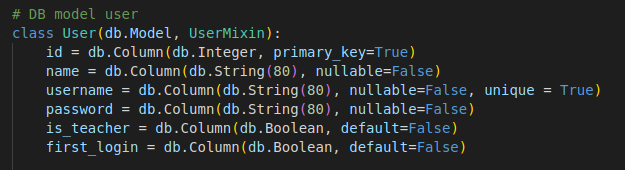
\includegraphics[scale=0.9]{img/imgs-memoria/UserModel.PNG}
    \caption{Modelo usuario}
\end{figure}

\subsection{Tablas de la base de datos}
Una vez obtenido un login funcional y como paso previo al desarrollo de las funcionalidades de la página, era necesaria la creación de las distintas tablas de base de datos las cuales nuestro futuro sistema dependería para funcionar, a excepción de la tabla usuarios la cual había sido requerida su implementación en el desarrollo del login. Esta taréa no fue de gran dificultad debido al fácil manejo que ofrece la herramienta SQLAlchemy y su utilización conjunta con Flask. 

La especificación concreta de tablas de la base de datos queda redactada en la sección \textit{C.2.Diseño de Datos} dentro del \textit{Anexo C: Especificación de diseño}.

\subsection{Funcionalidades para los alumnos}
Con las tablas necesarias para el funcionamiento de la plataforma ya creadas, el siguienta paso era la adición de todas las funcionalidades del alumno planeadas incialmente, las cuales consistían en: 
\begin{itemize}
\item Acceso a los cursos en los que el alumno está inscrito, junto con sus contenidos teóricos y tareas.
\item Entrega de las tareas resueltas y califición de forma automática.
\item Visualización de las calificaciones obtenidas en las tareas entregadas.
\item Cambio de contraseña.
\item Cierre de sesión.
\end{itemize}
Las anteriores funcionalidades descritas, a excepción de la entrega de tareas, fueron implementadas mediante funciones de Flask básicas. Sin embargo, para lograr la calificación automática de tareas tras la entrega de estas, fue necesaria la adaptación de la API pública de Nbgrader\cite{tool:NbgraderAPI} mediante una nueva clase dentro del proyecto denominada NbgraderManager, la cual sería completada posteriormente en el desarrollo de las funcionalidades para los profesores.

\subsection{Funcionalidades para los profesores}
Una vez añadidas las funcionalidades del alumno descritas en la sección anterior, llegaba el turno de los profesores. Estas funcionalidades iniciales eran las siguientes:
\begin{itemize}
\item Adición de cursos didáctivos y acceso a sus contenidos.
\item Creación de secciones de contenido dentro de un curso de forma directa (tarea creada previamente por el profesor de forma independiente).
\item Creación de secciones de contenido de forma indirecta (tarea creada desde la propia plataforma).
\item Consulta de calificaciones.
\item Inscripción y expulsión de alumnos en cursos.
\item Creación y eliminación de alumnos.
\item Cambio de contraseña.
\item Cierre de sesión.
\end{itemize}
Para las opciones de creación de secciones de contenido fue necesaria la adaptación de diversos métodos de la API de Nbgrader, completándose así la clase NbgraderManager mencionada con anterioridad. Adicionalmente, se adaptó el manejo de Jupyter Notebook dentro del código para hacer posible la edición de tareas desde la plataforma.

Debido a que nuestra plataforma no estaba orientada a contener usuarios de tipo administrador, en lo que respecta a la creación de nuevos alumnos se tomó la decisión de dejar esta tarea en manos de los profesores, quienes eligirían tanto nombre de usuario como contraseña para el alumno en cuestión. Con el fin de proteger la privacidad del alumno y darle a este la posibilidad de elegir su propia contraseña, cuando un alumno accede por primera vez a la plataforma con la contraseña escogida por el profesor, será direccionado de forma automática a la página de cambio de contraseña para que pueda escoger la contraseña de su cuenta personalmente, cambiando la dada incialmente por el profesor.
 
\subsection{Estilos y landing inicial}
Una vez completadas las funcionalidades inicialmente pensadas para profesores y alumnos, llegaba el momento de mejorar la estética de la plataforma, comenzando esta labor con la creación de un landing y, posteriormente, dando estilos al resto de vistas.

Los estilos del landing inicial y la página del login se dieron principalmente mediante CSS, a diferencia del resto de vistas las cuales recibieron sus estilos mediante la herramienta Bootstrap. Adicionalmente y con el objetivo de dar seguridad en la página frente a algunas acciones como el cierre de sesión, eliminación de alumnos o inscripción y baja de alumnos en cursos, fueron añadidas ventanas modales de confirmación de acciones mediante JavaScript.

Este proceso resultó un reto mayor de lo esperado dado que el presente Grado Universitado no profundiza demasiado en el manejo de estas herramientas. Por ello, fue necesario el estudio y práctica de estas herramientas hasta conseguir la adecuada soltura en su manejo.

\subsection{Adición de funcionalidades extra}
Tras finalizar la adición de estilos y con todas las funcionalidades previstas incialmente incluidas en la plataforma, surgió la necesidad de añadir nuevas opciones de funcionamiento debido a un mal diseño incial, que únicamente permitía la creación de cursos y secciones pero no su posterior eliminación. Junto a estas fueron añadidas otras funcionalidades orientadas al acceso a archivos relativos a las tareas y sus procesos de corrección automática:
\begin{itemize}
\item Eliminación de cursos existentes.
\item Eliminación de secciones de contenido de los cursos.
\item Descarga de los documentos tarea entregados por los alumnos.
\item Descarga de las tareas en versión profesor y alumno por parte de los profesores.
\item Posibilidad de publicación o cancelación de secciones aún no publicadas.
\item Descarga del estado actual de las tareas de las secciones aún no publicadas.
\item Descarga de documentos feedback de las tareas entregadas por parte de los alumnos.
\item Eliminación de calificaciones / entregas de tareas para permitir nuevos intentos.
\end{itemize}

La práctica en el manejo de Flask, Modales JS y adición de estilos conseguida durante el desarrollo de las funcionalidades previas hicieron de esta adición de nuevas funcionalidades una tarea mucho más sencilla en comparación con los retos a los que nos habíamos enfrentado con anterioridad.

\section{Despliegue}
Una vez finalizado el desarrollo de la plataforma y teniendo esta el funcionamiento esperado, llegaba el momento de su despliegue posibilitando el acceso al público a ella. Esto parecía que iba a resultar una tarea complicada y dilatada en el tiempo pero, gracias a la capa de servicios gratuita de Amazon Web Service (AWS), su realización fue más sencilla de lo esperado.

La profundización sobre el despliegue de la plataforma dentro de una instancia EC2 de AWS queda desarrollada en el \textit{Manual del Programador} incluido en el \textit{Anexo D: Documentación técnica de programación}.
\capitulo{6}{Trabajos relacionados}

Como se vio en los aspectos relavantes del desarrollo del proyecto, al realizar una investigación inicial acerca de las herramientas de autograding se descubrieron diversas plataformas orientadas a la corrección automática de ejercicios en lenguajes de programación como CodeGrade o CodingRooms. A continuación veremos otras plataformas y proyectos que siguen un formato similar:

\section{Plataformas}

\subsubsection{Codequiry}
Codequiry\cite{tool:Codequiry}\cite{tool:CodequiryAutograding} es una plataforma orientada a la detección de plagio de código la cual incluye, entre otras herramientas, la calificación de tareas de programación de forma automatizada, soportando hasta 20 lenguajes de programación distintos.
\begin{itemize}
\item \href{https://codequiry.com/}{Página oficial de Codequiry}
\item \href{https://codequiry.com/auto-grading-programming}{Sección orientada al autograding} 
\end{itemize}

\subsubsection{Codio}
Codio\cite{tool:Codio}\cite{tool:CodioAutograding} es una plataforma en la nube dedicada a la creación, calificación, testeo y calificación tanto manual como automática de tareas de programación.
La misión de Codio es la de impartir contenido educacional de alta calidad sobre la ciencia de datos, accesible por estudiantes de todo el mundo.
\begin{itemize}
\item \href{https://www.codio.com/}{Página oficial de Codio}
\item \href{https://www.codio.com/features/auto-grading}{Sección orientada al autograding}
\end{itemize}

\section{Proyectos}

\subsubsection{Desarrollo de un Sistema de Corrección Automática de Programas Haskell}
Se trata de un Trabajo de Fin de Grado realizado por Meritxell Sáez Povedano\cite{MeritxellSaezPovedano} en 2016 para la Universidad Politécnica de Valencia, orientado a la corrección automática de programas escritos en el lenguaje de programación Haskell.

A diferencia de nuestro proyecto el cual ha seguido una orientación didáctica basada en cursos, adaptando herramientas de autograding a dicho propósito, este proyecto optaba por la extensión del ya existente sistema de evaluación semi-automática de ejercicios en Java ''ASys''\cite{tool:ASys} con el fin de posibilitar la evaluación de ejercicios en Haskell.

\begin{itemize}
\item \href{http://personales.upv.es/josilga/ASys/about.html}{El sistema ASys}
\item \href{https://riunet.upv.es/handle/10251/72442?show=full}{Proyecto de Meritxell Sáez Povedano} 
\end{itemize}



\subsubsection{Aplicación web para el análisis automático de prácticas realizadas en el lenguaje Java}
Este es el Trabajo de Fin de Grado de Álvaro Vázquez\cite{AlvaroVazquez} para la Universidad de Burgos en 2019. En él se desarrolla una aplicación web de corrección automática de prácticas en el lenguaje Java ligada a la herramienta de gestión de aprendizaje Moodle, sistema muy similar al desarrollado en nuestro proyecto basado en un lenguaje de programación diferente.
\capitulo{7}{Conclusiones y Líneas de trabajo futuras}

Para dar cierre a esta memoria se expondrán en esta sección las conclusiones obtenidas tras el desarrollo del proyecto y posibles futuras líneas de trabajo a realizar.

\section{Conclusiones}
De este trabajo se han sacado las siguientes conclusiones:

\begin{itemize}
\item Se ha logrado el objetivo de desarrollar una plataforma orientada a la enseñanza a través de cursos con tareas en Python corregibles de forma automática, junto con la posibilidad de diseñar estas tareas desde la propia plataforma. Además se ha incluido en esta un pequeño curso introductorio sobre este lenguaje que permite a los alumnos adquirir los conocimientos necesarios para enfrentarse a los retos que podrían proponerse en los siguientes cursos añadidos a la plataforma. 
\item Se han adquirido conocimientos avanzados de manejo de diferentes herramientas orientadas al desarrollo web y autograding de tareas, combinándose estas con otras tecnologías con el objetivo de hacer frente a los diversos retos surgidos durante la realización del proyecto. 
\item El estudiante ha podido poner en práctica técnicas y conocimientos adquiridos a lo largo de su recorrido como estudiante del Grado en Ingeniería Informática de la Universidad de Burgos, enfrentándose a problemas de desarrollo reales y aportándole experiencia aplicable en futuros proyectos a los que tendrá que hacer frente.
\end{itemize}

\section{Líneas de trabajo futuras}
Tras la finalización del proyecto, quedan pendientes las siguientes líneas de trabajo:
\begin{itemize}
\item El hecho de que los profesores puedan editar tareas desde la propia plataforma mediante la ejecución remota de Jupyter Notebooks genera el problema de que estos puedan retroceder en el árbol de archivos de Jupyter, accediendo así a las carpetas de cursos de la plataforma. Queda establecida como posible línea de trabajo la resolución de este problema, el cual, en caso de ser resuelto, posibilitaría la opción de permitir a los alumnos resolver las tareas desde la propia plataforma.
\item En el estado actual en el que se encuentra la plataforma, esta no contiene ninguna forma de comunicación directa entre profesores y alumnos. Otra posible línea de trabajo sería la adición de algún sistema de comunicación entre estos, generándose así un ambiente de trato más personal dentro de la web. 
\item Actualmente no se han incluido marcas temporales para la entrega de tareas, funcionalidad que podría resultar de utilidad e interés dentro de la plataforma; es por ello por lo que se define esta como otra futura línea de trabajo.
\item Otra posible línea de trabajo derivable de este proyecto sería la adaptación de la plataforma web a la herramienta de gestión de aprendizaje Moodle \cite{Moodle}.
\end{itemize}

\bibliographystyle{plain}
\bibliography{bibliografia}


\end{document}
